\documentclass[english, 11 pt, class=article, crop=false]{standalone}
\usepackage[T1]{fontenc}
%\renewcommand*\familydefault{\sfdefault} % For dyslexia-friendly text
\usepackage{lmodern} % load a font with all the characters
\usepackage{geometry}
\geometry{verbose,paperwidth=16.1 cm, paperheight=24 cm, inner=2.3cm, outer=1.8 cm, bmargin=2cm, tmargin=1.8cm}
\setlength{\parindent}{0bp}
\usepackage{import}
\usepackage[subpreambles=false]{standalone}
\usepackage{amsmath}
\usepackage{amssymb}
\usepackage{esint}
\usepackage{babel}
\usepackage{tabu}
\makeatother
\makeatletter

\usepackage{titlesec}
\usepackage{ragged2e}
\RaggedRight
\raggedbottom
\frenchspacing

% Norwegian names of figures, chapters, parts and content
\addto\captionsenglish{\renewcommand{\figurename}{Figur}}
\makeatletter
\addto\captionsenglish{\renewcommand{\chaptername}{Kapittel}}
\addto\captionsenglish{\renewcommand{\partname}{Del}}


\usepackage{graphicx}
\usepackage{float}
\usepackage{subfig}
\usepackage{placeins}
\usepackage{cancel}
\usepackage{framed}
\usepackage{wrapfig}
\usepackage[subfigure]{tocloft}
\usepackage[font=footnotesize,labelfont=sl]{caption} % Figure caption
\usepackage{bm}
\usepackage[dvipsnames, table]{xcolor}
\definecolor{shadecolor}{rgb}{0.105469, 0.613281, 1}
\colorlet{shadecolor}{Emerald!15} 
\usepackage{icomma}
\makeatother
\usepackage[many]{tcolorbox}
\usepackage{multicol}
\usepackage{stackengine}

\usepackage{esvect} %For vectors with capital letters

% For tabular
\usepackage{array}
\usepackage{multirow}
\usepackage{longtable} %breakable table

% Ligningsreferanser
\usepackage{mathtools}
\mathtoolsset{showonlyrefs}

% index
\usepackage{imakeidx}
\makeindex[title=Indeks]

%Footnote:
\usepackage[bottom, hang, flushmargin]{footmisc}
\usepackage{perpage} 
\MakePerPage{footnote}
\addtolength{\footnotesep}{2mm}
\renewcommand{\thefootnote}{\arabic{footnote}}
\renewcommand\footnoterule{\rule{\linewidth}{0.4pt}}
\renewcommand{\thempfootnote}{\arabic{mpfootnote}}

%colors
\definecolor{c1}{cmyk}{0,0.5,1,0}
\definecolor{c2}{cmyk}{1,0.25,1,0}
\definecolor{n3}{cmyk}{1,0.,1,0}
\definecolor{neg}{cmyk}{1,0.,0.,0}

% Lister med bokstavar
\usepackage[inline]{enumitem}

\newcounter{rg}
\numberwithin{rg}{chapter}
\newcommand{\reg}[2][]{\begin{tcolorbox}[boxrule=0.3 mm,arc=0mm,colback=blue!3] {\refstepcounter{rg}\phantomsection \large \textbf{\therg \;#1} \vspace{5 pt}}\newline #2  \end{tcolorbox}\vspace{-5pt}}

\newcommand\alg[1]{\begin{align} #1 \end{align}}

\newcommand\eks[2][]{\begin{tcolorbox}[boxrule=0.3 mm,arc=0mm,enhanced jigsaw,breakable,colback=green!3] {\large \textbf{Eksempel #1} \vspace{5 pt}\\} #2 \end{tcolorbox}\vspace{-5pt} }

\newcommand{\st}[1]{\begin{tcolorbox}[boxrule=0.0 mm,arc=0mm,enhanced jigsaw,breakable,colback=yellow!12]{ #1} \end{tcolorbox}}

\newcommand{\spr}[1]{\begin{tcolorbox}[boxrule=0.3 mm,arc=0mm,enhanced jigsaw,breakable,colback=yellow!7] {\large \textbf{Språkboksen} \vspace{5 pt}\\} #1 \end{tcolorbox}\vspace{-5pt} }

\newcommand{\sym}[1]{\colorbox{blue!15}{#1}}

\newcommand{\info}[2]{\begin{tcolorbox}[boxrule=0.3 mm,arc=0mm,enhanced jigsaw,breakable,colback=cyan!6] {\large \textbf{#1} \vspace{5 pt}\\} #2 \end{tcolorbox}\vspace{-5pt} }

\newcommand\algv[1]{\vspace{-11 pt}\begin{align*} #1 \end{align*}}

\newcommand{\regv}{\vspace{5pt}}
\newcommand{\mer}{\textsl{Merk}: }
\newcommand{\mers}[1]{{\footnotesize \mer #1}}
\newcommand\vsk{\vspace{11pt}}
\newcommand\vs{\vspace{-11pt}}
\newcommand\vsb{\vspace{-16pt}}
\newcommand\sv{\vsk \textbf{Svar} \vspace{4 pt}\\}
\newcommand\br{\\[5 pt]}
\newcommand{\figp}[1]{../fig/#1}
\newcommand\algvv[1]{\vs\vs\begin{align*} #1 \end{align*}}
\newcommand{\y}[1]{$ {#1} $}
\newcommand{\os}{\\[5 pt]}
\newcommand{\prbxl}[2]{
\parbox[l][][l]{#1\linewidth}{#2
	}}
\newcommand{\prbxr}[2]{\parbox[r][][l]{#1\linewidth}{
		\setlength{\abovedisplayskip}{5pt}
		\setlength{\belowdisplayskip}{5pt}	
		\setlength{\abovedisplayshortskip}{0pt}
		\setlength{\belowdisplayshortskip}{0pt} 
		\begin{shaded}
			\footnotesize	#2 \end{shaded}}}

\renewcommand{\cfttoctitlefont}{\Large\bfseries}
\setlength{\cftaftertoctitleskip}{0 pt}
\setlength{\cftbeforetoctitleskip}{0 pt}

\newcommand{\bs}{\\[3pt]}
\newcommand{\vn}{\\[6pt]}
\newcommand{\fig}[1]{\begin{figure}
		\centering
		\includegraphics[]{\figp{#1}}
\end{figure}}

\newcommand{\figc}[2]{\begin{figure}
		\centering
		\includegraphics[]{\figp{#1}}
		\caption{#2}
\end{figure}}

\newcommand{\sectionbreak}{\clearpage} % New page on each section

\newcommand{\nn}[1]{
\begin{equation}
	#1
\end{equation}
}

% Equation comments
\newcommand{\cm}[1]{\llap{\color{blue} #1}}

\newcommand\fork[2]{\begin{tcolorbox}[boxrule=0.3 mm,arc=0mm,enhanced jigsaw,breakable,colback=yellow!7] {\large \textbf{#1 (forklaring)} \vspace{5 pt}\\} #2 \end{tcolorbox}\vspace{-5pt} }
 
%colors
\newcommand{\colr}[1]{{\color{red} #1}}
\newcommand{\colb}[1]{{\color{blue} #1}}
\newcommand{\colo}[1]{{\color{orange} #1}}
\newcommand{\colc}[1]{{\color{cyan} #1}}
\definecolor{projectgreen}{cmyk}{100,0,100,0}
\newcommand{\colg}[1]{{\color{projectgreen} #1}}

% Methods
\newcommand{\metode}[2]{
	\textsl{#1} \\[-8pt]
	\rule{#2}{0.75pt}
}

%Opg
\newcommand{\abc}[1]{
	\begin{enumerate}[label=\alph*),leftmargin=18pt]
		#1
	\end{enumerate}
}
\newcommand{\abcs}[2]{
	\begin{enumerate}[label=\alph*),start=#1,leftmargin=18pt]
		#2
	\end{enumerate}
}
\newcommand{\abcn}[1]{
	\begin{enumerate}[label=\arabic*),leftmargin=18pt]
		#1
	\end{enumerate}
}
\newcommand{\abch}[1]{
	\hspace{-2pt}	\begin{enumerate*}[label=\alph*), itemjoin=\hspace{1cm}]
		#1
	\end{enumerate*}
}
\newcommand{\abchs}[2]{
	\hspace{-2pt}	\begin{enumerate*}[label=\alph*), itemjoin=\hspace{1cm}, start=#1]
		#2
	\end{enumerate*}
}

% Oppgaver
\newcommand{\opgt}{\phantomsection \addcontentsline{toc}{section}{Oppgaver} \section*{Oppgaver for kapittel \thechapter}\vs \setcounter{section}{1}}
\newcounter{opg}
\numberwithin{opg}{section}
\newcommand{\op}[1]{\vspace{15pt} \refstepcounter{opg}\large \textbf{\color{blue}\theopg} \vspace{2 pt} \label{#1} \\}
\newcommand{\ekspop}[1]{\vsk\textbf{Gruble \thechapter.#1}\vspace{2 pt} \\}
\newcommand{\nes}{\stepcounter{section}
	\setcounter{opg}{0}}
\newcommand{\opr}[1]{\vspace{3pt}\textbf{\ref{#1}}}
\newcommand{\oeks}[1]{\begin{tcolorbox}[boxrule=0.3 mm,arc=0mm,colback=white]
		\textit{Eksempel: } #1	  
\end{tcolorbox}}
\newcommand\opgeks[2][]{\begin{tcolorbox}[boxrule=0.1 mm,arc=0mm,enhanced jigsaw,breakable,colback=white] {\footnotesize \textbf{Eksempel #1} \\} \footnotesize #2 \end{tcolorbox}\vspace{-5pt} }
\newcommand{\rknut}{
Rekn ut.
}

%License
\newcommand{\lic}{\textit{Matematikken sine byggesteinar by Sindre Sogge Heggen is licensed under CC BY-NC-SA 4.0. To view a copy of this license, visit\\ 
		\net{http://creativecommons.org/licenses/by-nc-sa/4.0/}{http://creativecommons.org/licenses/by-nc-sa/4.0/}}}

%referances
\newcommand{\net}[2]{{\color{blue}\href{#1}{#2}}}
\newcommand{\hrs}[2]{\hyperref[#1]{\color{blue}\textsl{#2 \ref*{#1}}}}
\newcommand{\rref}[1]{\hrs{#1}{regel}}
\newcommand{\refkap}[1]{\hrs{#1}{kapittel}}
\newcommand{\refsec}[1]{\hrs{#1}{seksjon}}

\newcommand{\mb}{\net{https://sindrsh.github.io/FirstPrinciplesOfMath/}{MB}}


%line to seperate examples
\newcommand{\linje}{\rule{\linewidth}{1pt} }

\usepackage{datetime2}
%%\usepackage{sansmathfonts} for dyslexia-friendly math
\usepackage[]{hyperref}


\begin{document}
\opgt

\op{geo1}
Finn den siste vinkelen i trekanten når de to andre vinklene er:\os
\begin{tabular}{@{}l l l l}
	\textbf{a)} $ 60^\circ $ og $ 37^\circ $
	&	\textbf{b)} $ 90^\circ $ og $ 15^\circ $
	&	\textbf{b)} $ 45^\circ $ og $ 45^\circ $
	&	\textbf{b)} $ 60^\circ $ og $ 30^\circ $
\end{tabular}

\op{geo2}
Forklar hvorfor:\os
\textbf{a)} $ \triangle ABC $ og $ \triangle DEF $ er formlike.\\
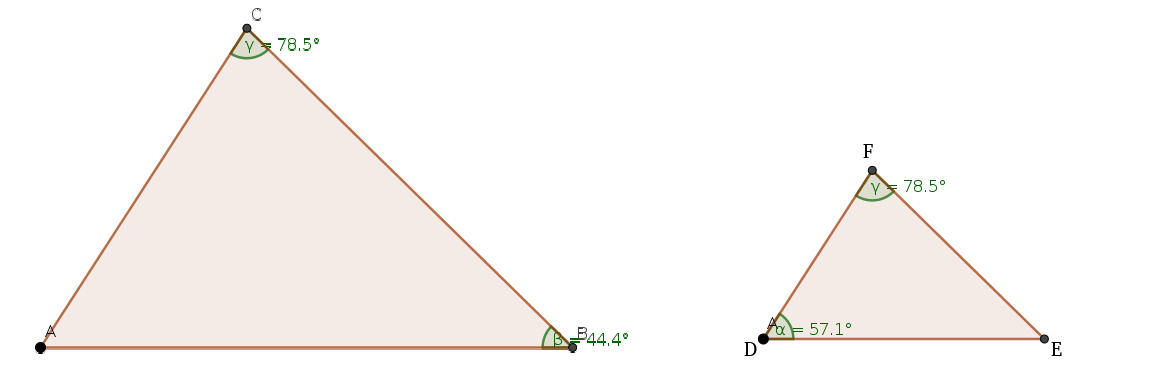
\includegraphics[scale=0.5]{frm1}


\textbf{b)} $ \triangle ABC$ og $ \triangle DBE $ er formlike. ($ AC $ og $ DE $ er parallelle).\\
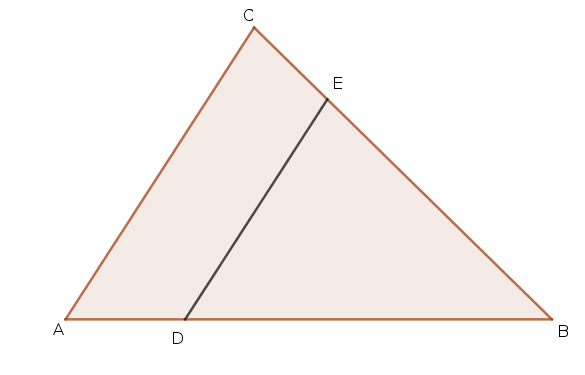
\includegraphics[scale=0.5]{frm2}.
\newpage
\textbf{c)} $ \triangle ABC$ og $ \triangle ADC $ er formlike.\\
\fig{tri4}

\nes
\nes
\op{geo0}
Trekantene under er formlike og $ AB $ er samsvarende med $ DE $.
\begin{figure}
	\centering
	\includegraphics[scale=1]{\asym{tri7a}}\qquad
	\includegraphics[scale=1]{\asym{tri7b}}
\end{figure}
Finn lengden til $ EF $ og $ AC $.

\op{geo3} Se tilbake til oppgave \ref{geo2}c. \os
\textbf{a)} Hvilke sider i $\triangle ABC$ og $ \triangle ADC $ er samsvarende sider? (Svaret \textsl{må} begrunnes!).\os
\textbf{b)} Vi har at $ {AC=4} $ og $ {AD=3,2} $. Finn lengden til $ AB $.  \os
\textbf{c)} Videre har vi at $ {BC=3} $. Finn lengden til $ CD $.

\op{geo4}
På en solrik dag får du kjæresten din, som viser seg å være en 2\,m høy bikinidame, til å stille seg i skyggen av en palme slik at solstrålen såvidt sneier det gyldne håret hennes.
\begin{figure}
	\centering
	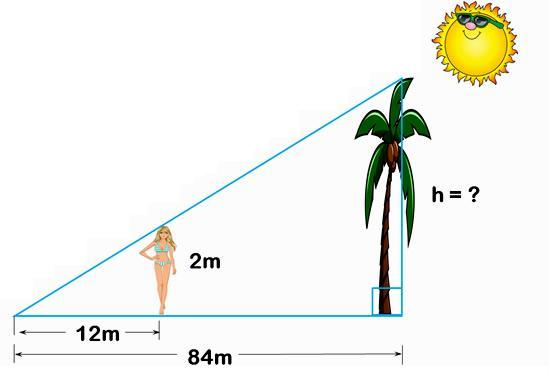
\includegraphics[scale=0.4]{bikini}
	\footnotesize\\
	\textit{kilde: \url{http://passyworldofmathematics.com/similar-triangles-applications/}}
\end{figure}
Hvor høy er palmen?

\op{geo5}
Trekantene $ \angle ABC $ og $ \triangle DEF $ er formlike. $ AB $ og $ DE $ er samsvarende sider og $ \frac{AB}{DF}=2 $, i tillegg er $ {BC=8, EF=4,5}  $ og $ {DF=4} $. Er $ BC $ samsvarende med $ EF $ eller $ DF $?
\vspace{15pt}

\nes
\nes
\nes
\nes
\nes
\op{geo6}
Finn lengden til $ x $:\os
\textbf{a)}\vsb
\fig{tri27a}
\textbf{b)} \vsb
\fig{tri27}
\textbf{c)}\vsb
\fig{tri27b}
\newpage
\op{geo7} 
(Oppgaven er hentet fra eksamen i 2015).\os
Et vindu har form som et rektangel. Vinduet er 6\,dm bredt og 7\,dm høyt. Gjør beregninger og avgjør om det er mulig å få en kvadratisk plate med sider 9 dm inn
gjennom vinduet.\os

\op{geo8}
Hvordan kan du sjekke om en trekant er rettvinklet eller ikke?

\op{geo9}
(Oppgaven er hentet fra eksamen i 2017).\\
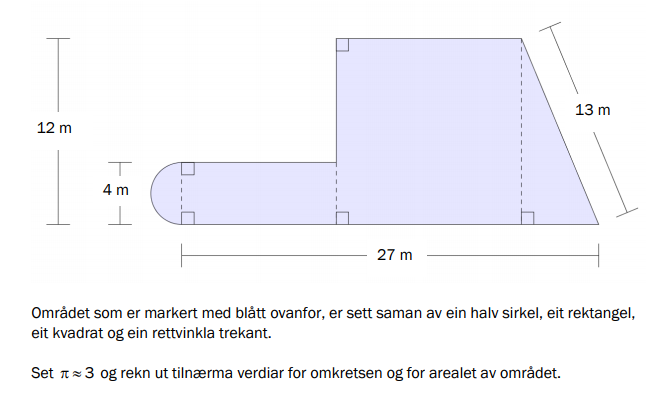
\includegraphics[scale=0.55]{eksv17}

\newpage
\op{geo10}
(Denne oppgaven har jeg fått av en veiarbeider som faktisk satt med akkurat dette problemet på jobben.)\os
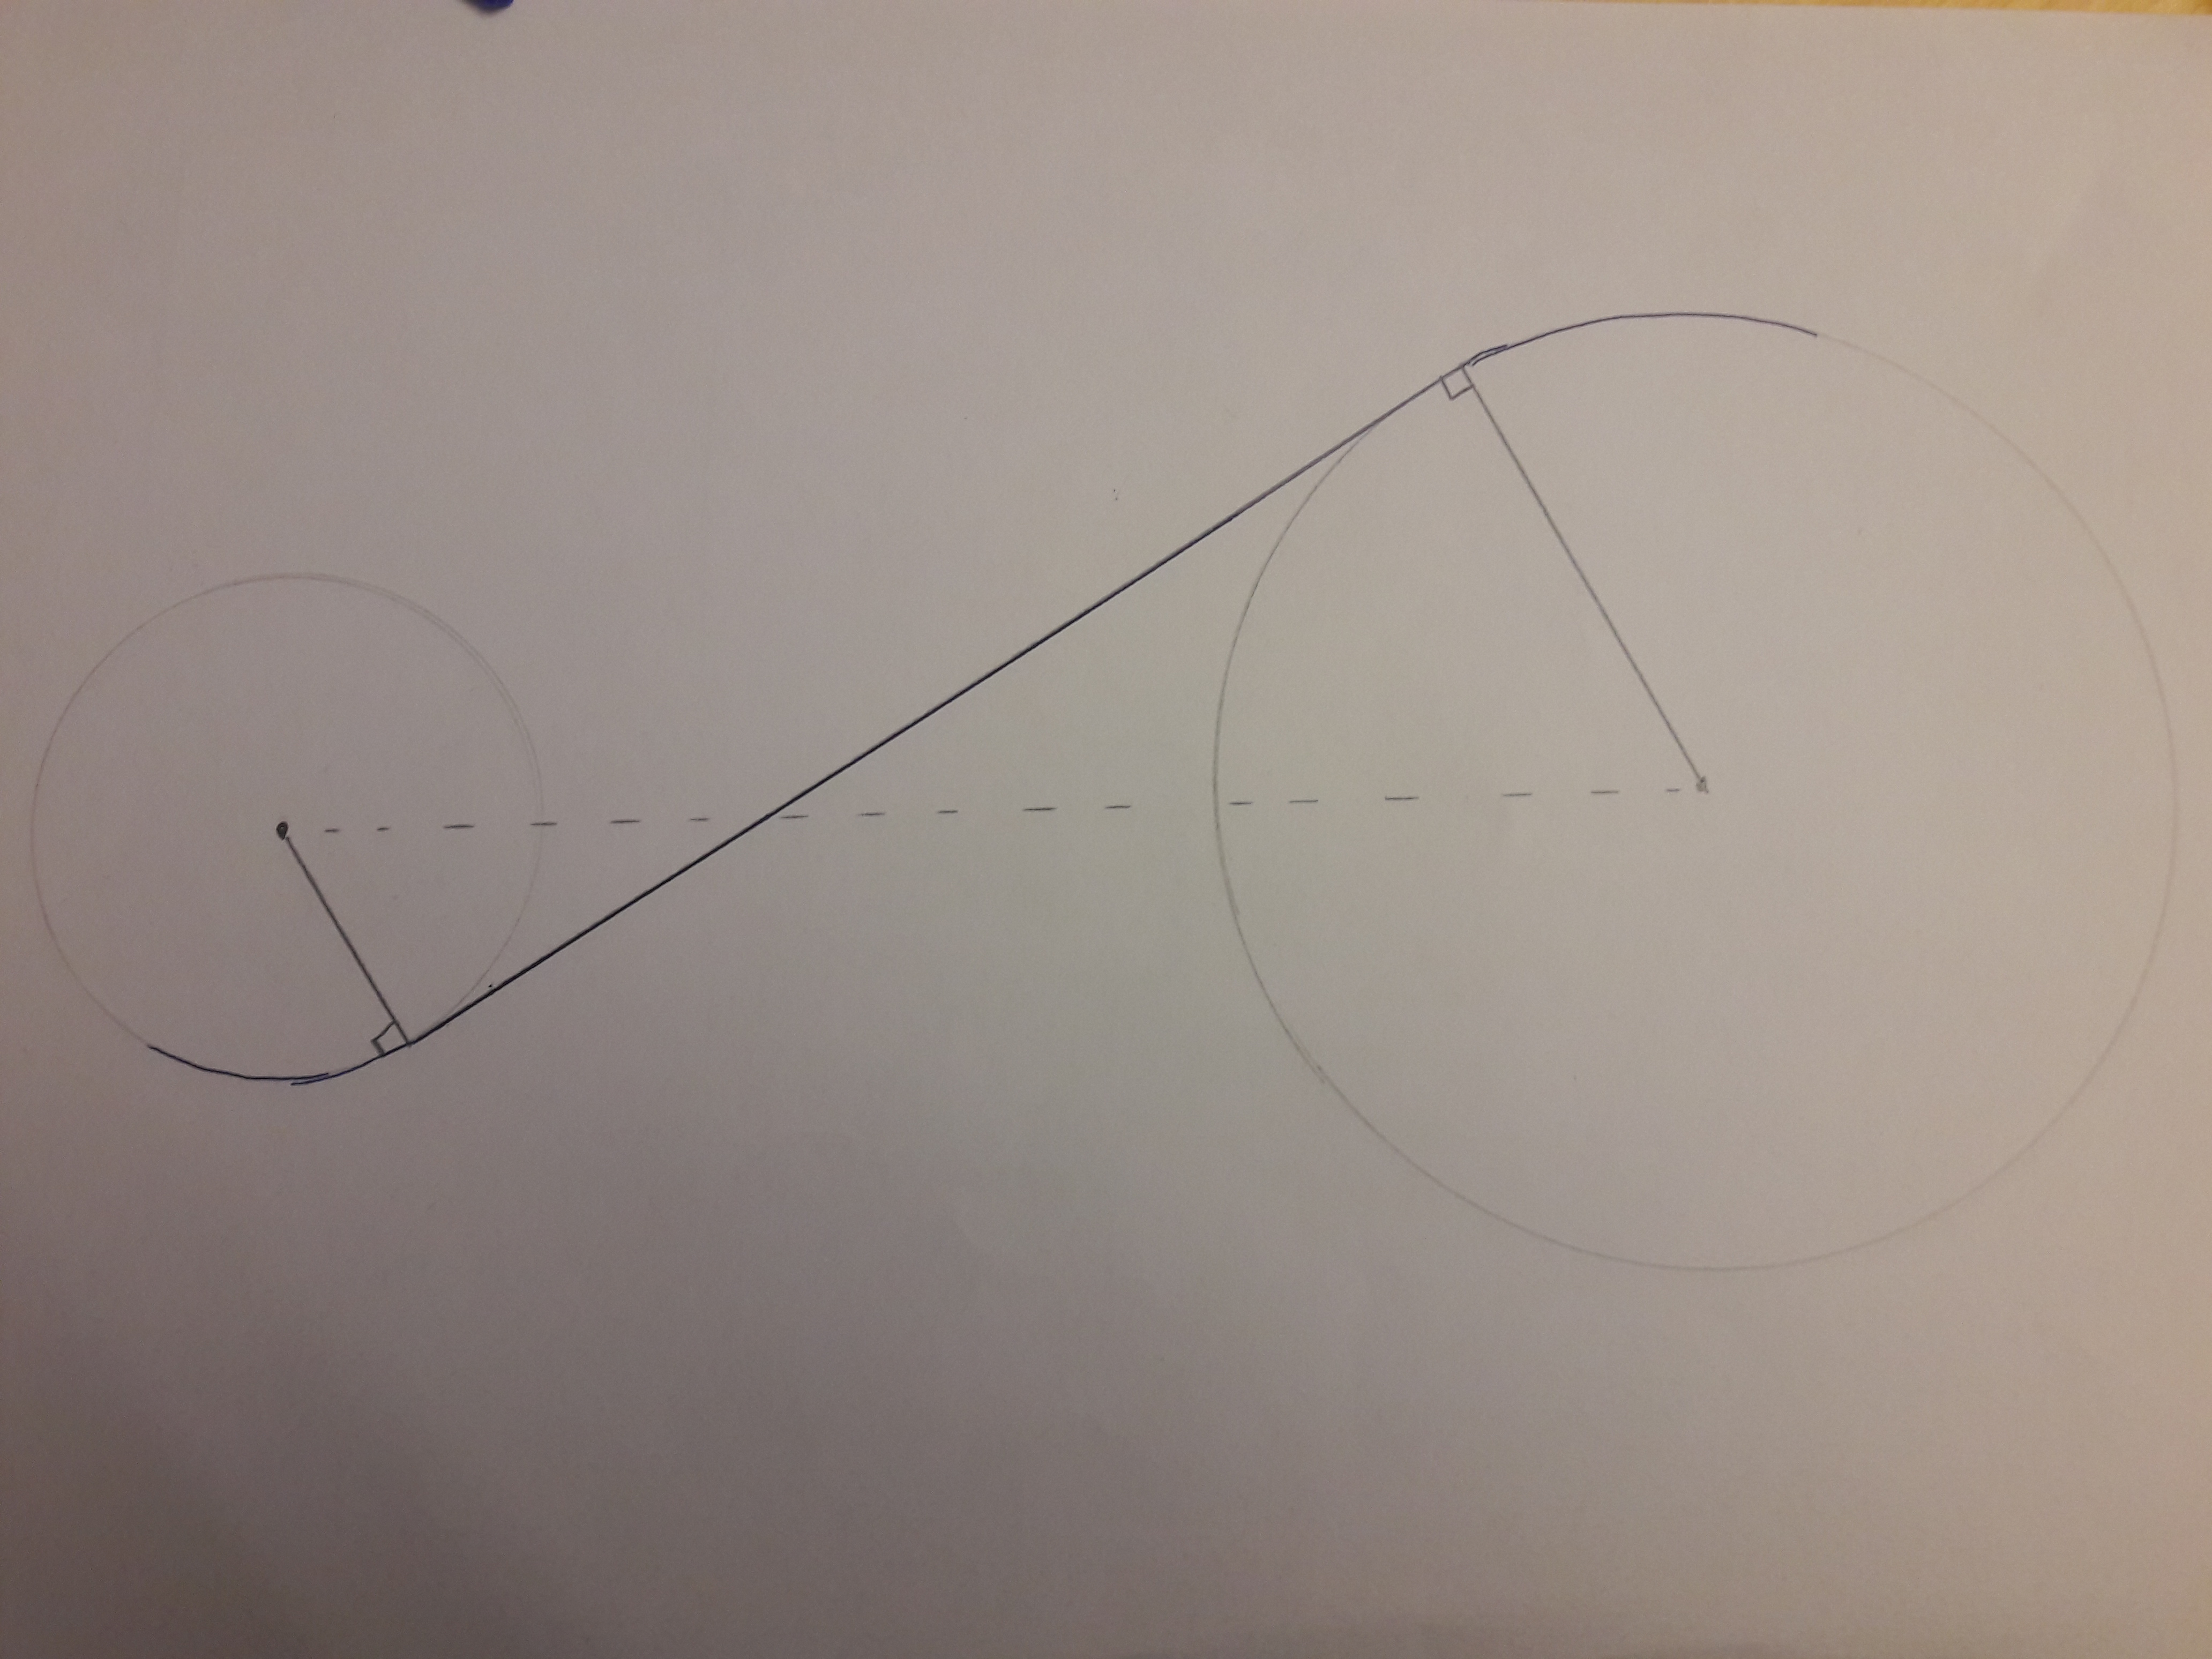
\includegraphics[scale=0.07]{vei}\os
En vei (den mørke linjen) skal komme fra en liten sving (til venstre) og etterpå kjøre et rett strekke til den kommer inn i en ny og større sving (til høyre).\os
Den lille radiusen er 30\,m, den store er 60\,m og den stiplete avstanden er 170,5\,m. Hvor langt er det rette veistrekket?
\nes

\op{geo11}
Finn volumet av:\os
	\textbf{a)} En firkantet boks med bredde 5, lengde 2 og høyde 11. \os
\textbf{b)} En sylinder med radius 4 og høyde 7 (bruk at $ \pi\approx 3 $).\os
\textbf{c)} En kjegle med radius 2 og høyde 9.\os
\textbf{d)} En pyramide med bredde 10, lengde 3 og høyde 2.
\newpage
\op{geo12}
(Hentet fra eksamen høsten 2017, del 1 (altså med hjelpemidler)
\begin{figure}
	\centering
	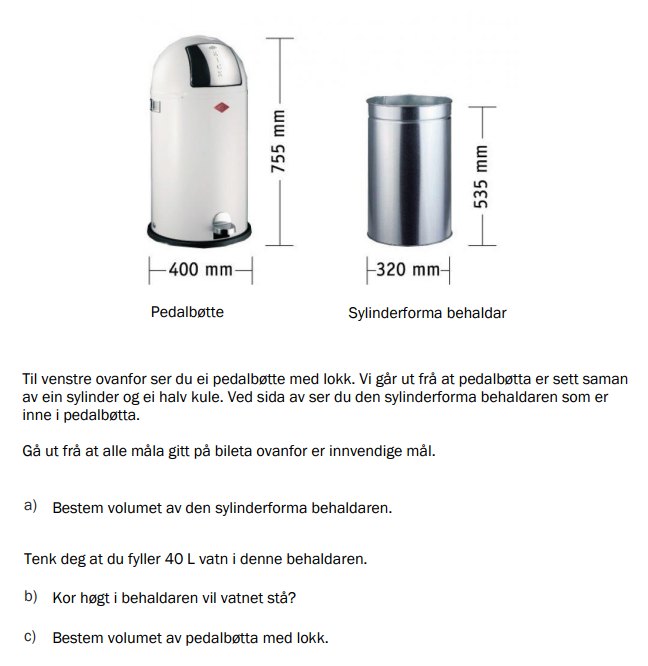
\includegraphics[scale=0.6]{eks17_2}
\end{figure}
\newpage
\op{geo13}
(Hentet fra eksamen høsten 2016, del 2 (altså med hjelpemidler))
\begin{figure}
	\centering
	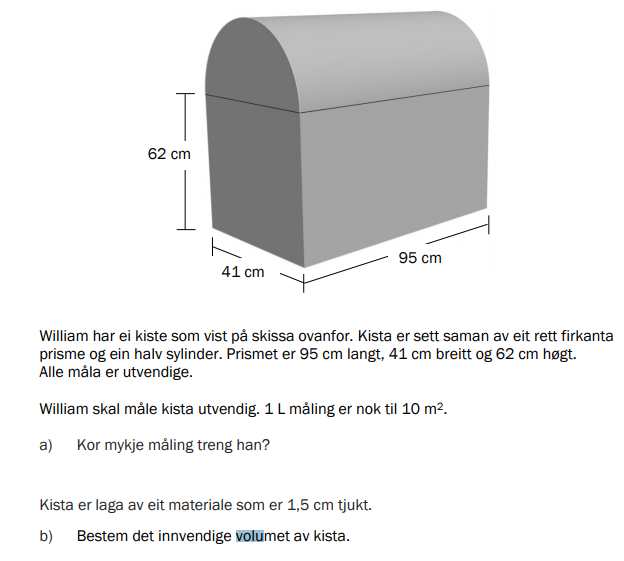
\includegraphics[scale=0.6]{eks_16_5}
\end{figure}

\newpage
{\color{blue}\textbf{Grubleoppgave}}\\ \vspace{2pt}
I denne oppgaven skal vi komme fram til en av de mest kjente læresetningene i geometri.
\fig{tri5}
Vi tar utgangspunkt i en hvilken som helst trekant $ \triangle ABC $ med $ {\angle ACB=90^\circ} $. På siden $ AB $ markerer vi punktet $ D $ som er slik at $ CD $ står vinkelrett på $ AB $. Da blir (se opg. \ref{geo2}c) $ \triangle ABC $, $ \triangle ADC$ og $ \triangle DBC $ alle sammen formlike. For å unngå drøssevis av store bokstaver sier vi videre at:
\[ \begin{matrix}
BC = a, & AC=b,& AB=c, & DB=x ,&  AD=c-x 
\end{matrix} \]
Målet vårt er nå å lage en formel som gjør at vi kan finne lengden til $ c $ hvis vi kjenner lengden til $ a $ og $ b $.\os
\textbf{a)} 
Finn sidene i $ \triangle ABC $ som samsvarer med sidene $ x $ og $ a $ i $ \triangle DBC $. Skriv formelen som viser forholdet mellom disse sidene.\os

\textbf{b)} Finn sidene i $ \triangle ABC $ som samsvarer med sidene $ b $ og $ {c-x} $ i $ \triangle ADC $. Skriv formelen som viser forholdet mellom disse sidene.\os
\textbf{c)} Skriv om formelen du fant i opg. a) til en formel for $ {c\cdot x} $.\os
\textbf{d)} Skriv om formelen du fant i opg. b) til en formel for $ {c^2-c\cdot x}  $.\os
\textbf{e)} Erstatt $ c\cdot x $ fra opg. d) med formelen du fant i oppgave c). Skriv om formelen slik at alle $ c $-er står på én side. Hvilken formel får du da?
\begin{comment}
\alg{
\frac{x}{a}=\frac{a}{c} \br
\frac{c-x}{b}=\frac{b}{c} \br
cx = a^2 \br
c^2-cx &= b^2
}
\end{comment}

\end{document}

